\documentclass[sigplan,screen]{acmart}
\usepackage[utf8]{inputenc}
\usepackage{microtype}
\usepackage{hyphenat}
\usepackage{amssymb}
\usepackage{tikz}
\usetikzlibrary{arrows.meta,positioning,shapes.geometric,calc,fit,backgrounds}

\definecolor{pipIndigo}{RGB}{79,70,229}
\definecolor{pipIndigoFill}{RGB}{238,242,255}
\definecolor{pipRed}{RGB}{220,38,38}
\definecolor{pipRedFill}{RGB}{254,242,242}
\definecolor{pipCyan}{RGB}{8,145,178}
\definecolor{pipCyanFill}{RGB}{236,254,255}
\definecolor{pipViolet}{RGB}{124,58,237}
\definecolor{pipVioletFill}{RGB}{245,243,255}
\definecolor{pipGreen}{RGB}{22,163,74}
\definecolor{pipGreenFill}{RGB}{240,253,244}
\definecolor{pipAmber}{RGB}{180,83,9}
\definecolor{pipAmberFill}{RGB}{255,251,235}
\definecolor{pipOrange}{RGB}{234,88,12}
\definecolor{pipOrangeFill}{RGB}{255,247,237}

%%% The following is specific to SPLASH '26 and the paper
%%% 'Slice-Guided, Context-Augmented Large Language Model Inference of Java Nullability Annotations'
%%% by Mushfiqur Rahman Chowdhury.
%%%
\setcopyright{cc}
\setcctype{by}
\acmDOI{10.1145/3837729.3839583}
\acmYear{2026}
\copyrightyear{2026}
\acmISBN{979-8-4007-2910-2/2026/10}
\acmConference[SPLASH Companion '26]{Companion Proceedings of the 2026 ACM SIGPLAN International Conference on Systems, Programming, Languages, and Applications: Software for Humanity}{October 4--9, 2026}{Oakland, CA, USA}
\acmBooktitle{Companion Proceedings of the 2026 ACM SIGPLAN International Conference on Systems, Programming, Languages, and Applications: Software for Humanity (SPLASH Companion '26), October 4--9, 2026, Oakland, CA, USA}
\acmSubmissionID{splashcomp26src-p21-p}
\received{2026-06-27}
\received[accepted]{2026-07-25}

\begin{document}

\title[Slice-Guided, Context-Augmented Large Language Model Inference \ldots]{
  Slice-Guided, Context-Augm\-ented Large Language Model Inference of Java Nullability Annotations}

\author{Mushfiqur Rahman Chowdhury}
\orcid{0009-0004-4461-8467}
\affiliation{%
  \institution{New Jersey Institute of Technology}
  \city{New Jersey}
  \country{USA}
}
\email{mc2399@njit.edu}

\begin{abstract}
Java nullness checkers such as NullAway catch potential null-pointer errors, but adopting them on legacy code is difficult. Most projects lack complete nullability annotations, and existing tools such as NullAwayAnnotator are checker-specific and can still leave warnings behind. We present a warning-guided, slice-based, LLM-assisted pipeline for inferring Java nullability annotations. It first runs NullAway to locate the warnings, then uses Specimin, a \emph{type-directed slicer} that extracts the minimum compilable code needed to reproduce a warning, to build a small slice around each warning-relevant method or field. It augments the prompt with \emph{usage context}. The model gets two complementary inputs, the compilable slice and this textual evidence, and infers the annotations \texttt{@Nullable} and \texttt{@Nonnull} without touching program logic. Annotations are merged back, re-checked, and a  post-processing loop fixes whatever still triggers a warning. On EventBus, where NullAwayAnnotator leaves 11 warnings unresolved, our pipeline resolves all warnings. We see this checker-guided design as a step toward a type-system-independent inference technique.
\end{abstract}

%% CCS Concepts: generate the verified snippet at https://dl.acm.org/ccs (search the
%% category names below, or better ones, and paste the tool's exact XML block) before
%% final submission. The first concept_id is a commonly used, high-confidence ID; the
%% remaining two are placeholders and MUST be replaced with the tool's exact IDs.
\begin{CCSXML}
<ccs2012>
<concept>
<concept_id>10011007.10010940.10010992.10010998.10011000</concept_id>
<concept_desc>Software and its engineering~Automated static analysis</concept_desc>
<concept_significance>500</concept_significance>
</concept>
<concept>
<concept_id>10003752.10010124.10010138.10010143</concept_id>
<concept_desc>Theory of computation~Program analysis</concept_desc>
<concept_significance>500</concept_significance>
</concept>
<concept>
<concept_id>10011007.10011074.10011099.10011102.10011103</concept_id>
<concept_desc>Software and its engineering~Software testing and debugging</concept_desc>
<concept_significance>300</concept_significance>
</concept>
</ccs2012>
\end{CCSXML}

\ccsdesc[500]{Software and its engineering~Automated static analysis}
\ccsdesc[500]{Theory of computation~Program analysis}
\ccsdesc[300]{Software and its engineering~Software testing and debugging}


\keywords{Nullability annotations, Static analysis, Large language models, Program slicing, Java}

\maketitle

\section{Introduction}

Null-pointer errors remain a common source of Java reliability bugs. Static nullness checkers such as NullAway~\cite{banerjee2019nullaway}, the Checker Framework Nullness Checker~\cite{papi2008practical}, and Meta's NullSafe~\cite{meta_nullsafe} catch potential null dereferences, but only as well as the annotations in the code allow. Incomplete or missing annotations mean retrofitting them by hand requires understanding usage patterns across the whole codebase which is a real barrier to adoption.

A few tools automate this. NullAwayAnnotator~\cite{karimipour2023practical} performs iterative, search-based inference for NullAway, and learning-based approaches such as NullGTN~\cite{siddiqui2024inferring} and NullRepair~\cite{karimipour2025llm} predict or repair nullability directly. All are nullability-specific. The Checker Framework's whole-program inference ("WPI")~\cite{kellogg2023pluggable} is the only technique not tied to a single property, but a recent comparison~\cite{karimipour2025new} found it infers nullability poorly.

LLMs look attractive here, but handing one an entire repository is impractical, and a recent baseline shows unconstrained prompting yields limited accuracy~\cite{karimipour2025llm}. We instead treat the LLM as a constrained component inside a static-analysis feedback loop. NullAway points to where annotations are needed, Specimin~\cite{nguyen2025static} extracts the minimum compilable code needed to trigger each warning, turning one repository-scale problem into many small, checkable ones that fit an LLM's context window. 

% ----------------------------------------------------------------------
\begin{figure}[t]
  \centering
  \resizebox{\columnwidth}{!}{%
  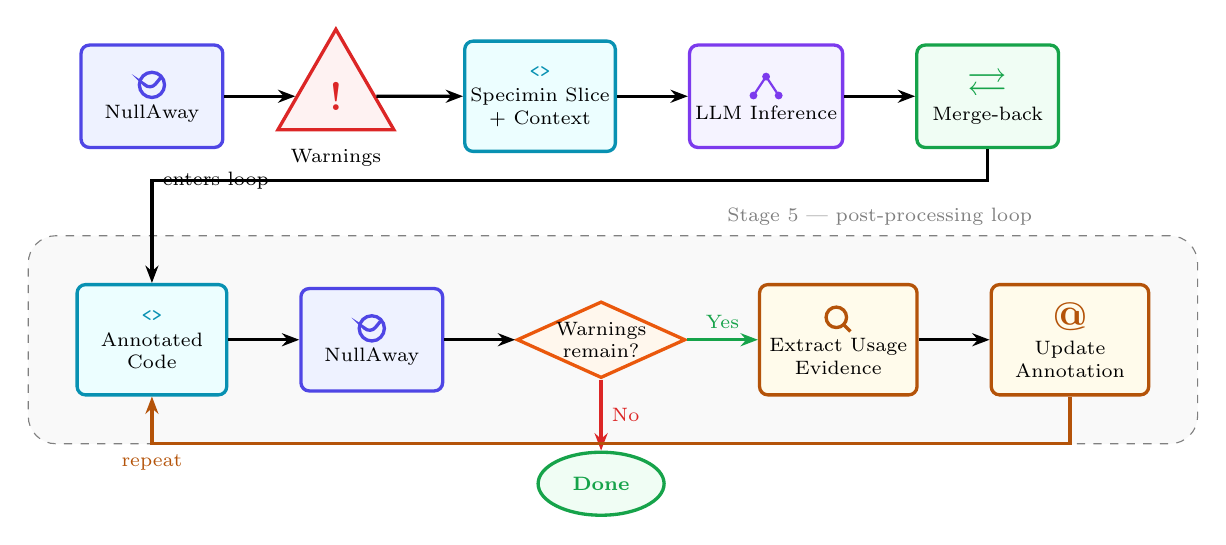
\begin{tikzpicture}[
      napbox/.style={rectangle, rounded corners=3pt, draw=pipIndigo, very thick,
        fill=pipIndigoFill, minimum width=18mm, minimum height=13mm,
        align=center, inner sep=2pt, font=\scriptsize},
      codebox/.style={rectangle, rounded corners=3pt, draw=pipCyan, very thick,
        fill=pipCyanFill, minimum width=19mm, minimum height=14mm,
        align=center, inner sep=2pt, font=\scriptsize},
      llmbox/.style={rectangle, rounded corners=3pt, draw=pipViolet, very thick,
        fill=pipVioletFill, minimum width=18mm, minimum height=13mm,
        align=center, inner sep=2pt, font=\scriptsize},
      mergebox/.style={rectangle, rounded corners=3pt, draw=pipGreen, very thick,
        fill=pipGreenFill, minimum width=18mm, minimum height=13mm,
        align=center, inner sep=2pt, font=\scriptsize},
      evidbox/.style={rectangle, rounded corners=3pt, draw=pipAmber, very thick,
        fill=pipAmberFill, minimum width=20mm, minimum height=14mm,
        align=center, inner sep=2pt, font=\scriptsize},
      warnshape/.style={regular polygon, regular polygon sides=3,
        draw=pipRed, very thick, fill=pipRedFill, minimum size=17mm,
        inner sep=0pt},
      decshape/.style={diamond, draw=pipOrange, very thick, fill=pipOrangeFill,
        aspect=2.2, align=center, inner sep=0pt, font=\scriptsize},
      termshape/.style={ellipse, draw=pipGreen, very thick, fill=pipGreenFill,
        align=center, inner sep=2pt, font=\scriptsize,
        minimum width=16mm, minimum height=8mm},
      pipcap/.style={font=\scriptsize, text=black},
      arr/.style={-{Stealth[length=2.2mm]}, very thick},
      elbl/.style={font=\scriptsize, midway},
    ]
    % ---- Row 1: warning-guided slicing and inference ----
    \node[napbox] (na1)
      {\tikz[baseline=-0.5ex]{
         \draw[very thick, pipIndigo] (0,0) circle (1.6mm);
         \draw[very thick, pipIndigo] (-0.9mm,0mm) -- (-0.2mm,-0.7mm) -- (1.1mm,0.9mm);
       }\\[1pt] NullAway};
    \node[warnshape, right=9mm of na1] (warn) {\Large\textbf{\textcolor{pipRed}{!}}};
    \node[pipcap, below=1mm of warn] (warnlbl) {Warnings};
    \node[codebox, right=11mm of warn] (slice)
      {\texttt{\textcolor{pipCyan}{<>}}\\[1pt] Specimin Slice\\ + Context};
    \node[llmbox, right=9mm of slice] (llm)
      {\tikz[baseline=-0.5ex]{
         \fill[pipViolet] (0,1.8mm) circle (0.5mm);
         \fill[pipViolet] (-1.6mm,-0.6mm) circle (0.5mm);
         \fill[pipViolet] (1.6mm,-0.6mm) circle (0.5mm);
         \draw[pipViolet, thick] (0,1.8mm) -- (-1.6mm,-0.6mm);
         \draw[pipViolet, thick] (0,1.8mm) -- (1.6mm,-0.6mm);
       }\\[1pt] LLM Inference};
    \node[mergebox, right=9mm of llm] (merge)
      {\textcolor{pipGreen}{\Large $\rightleftarrows$}\\[1pt] Merge-back};

    \draw[arr] (na1) -- (warn);
    \draw[arr] (warn) -- (slice);
    \draw[arr] (slice) -- (llm);
    \draw[arr] (llm) -- (merge);

    % ---- Row 2: evidence-driven post-processing loop ----
    \node[codebox, below=17mm of na1] (acode)
      {\texttt{\textcolor{pipCyan}{<>}}\\[1pt] Annotated\\ Code};
    \node[napbox, right=9mm of acode] (na2)
      {\tikz[baseline=-0.5ex]{
         \draw[very thick, pipIndigo] (0,0) circle (1.6mm);
         \draw[very thick, pipIndigo] (-0.9mm,0mm) -- (-0.2mm,-0.7mm) -- (1.1mm,0.9mm);
       }\\[1pt] NullAway};
    \node[decshape, right=9mm of na2] (dec) {Warnings\\ remain?};
    \node[evidbox, right=9mm of dec] (extr)
      {\tikz[baseline=-0.5ex]{
         \draw[very thick, pipAmber] (0,0.3mm) circle (1.3mm);
         \draw[very thick, pipAmber] (0.9mm,-0.6mm) -- (1.8mm,-1.5mm);
       }\\[1pt] Extract Usage\\ Evidence};
    \node[evidbox, right=9mm of extr] (upd)
      {\textcolor{pipAmber}{\Large\textbf{@}}\\[1pt] Update\\ Annotation};
    \node[termshape, below=9mm of dec] (done) {\textbf{\textcolor{pipGreen}{Done}}};

    \draw[arr] (acode) -- (na2);
    \draw[arr] (na2) -- (dec);
    \draw[arr, draw=pipGreen] (dec) -- node[elbl, above, text=pipGreen]{Yes} (extr);
    \draw[arr, draw=pipRed] (dec) -- node[elbl, right, text=pipRed]{No} (done);
    \draw[arr] (extr) -- (upd);
    \draw[arr, draw=pipAmber] (upd.south) -- ++(0,-6mm) -|
      node[elbl, below, text=pipAmber]{repeat} (acode.south);
    \draw[arr] (merge.south) -- ++(0,-4mm) -|
      node[elbl, right]{enters loop} (acode.north);

    \begin{scope}[on background layer]
      \node[draw=gray, dashed, rounded corners=10pt, fill=gray!5,
        fit=(acode)(na2)(dec)(extr)(upd), inner sep=6mm,
        label={[gray,font=\scriptsize]above right:Stage 5 --- post-processing loop}]
        {};
    \end{scope}
  \end{tikzpicture}%
  }
  \caption{Pipeline overview. NullAway warnings drive Specimin to extract a
minimal slice and usage context; an LLM infers
\texttt{@Nullable}/\texttt{@Nonnull} on the slice, the annotations merge
back, and the post-processing loop re-checks with NullAway and corrects
annotations from the evidence until none remain.}
  \label{fig:approach}
\end{figure}
% ----------------------------------------------------------------------

\section{Approach and Implementation}
\label{sec:approach}

The pipeline runs in five stages (Figure~\ref{fig:approach}). (1)~\emph{Warning extraction} runs NullAway on the project and parses its output to locate each warning's target method or field. (2)~\emph{Slicing} invokes Specimin on each target to produce a reduced, compilable Java slice. (3)~\emph{Constrained inference} prompts the LLM with the slice, its warnings, and usage context to decide nullability for each parameter, return type, and field, emitting files that use only \texttt{Nullable}/\texttt{Nonnull} and change nothing else. (4)~\emph{Merge-back} projects the annotations into the original repository and reruns NullAway. (5)~A \emph{post-processing loop} re-runs NullAway and corrects whichever annotations are still responsible for a warning (described below).

\paragraph{Type-Directed Slicing with Specimin.}
Specimin~\cite{nguyen2025static} is a \emph{type-directed program slicer}. Given a program and target methods or fields, it produces a small compilable program that preserves the declared types and signatures those targets depend on, stubbing out everything else's body. The result is a self-contained reproduction of the warning that NullAway can run on directly.

\paragraph{Usage Context.}
Specimin's stubbing can remove important usage context for fields, including dereferences, null guards (\texttt{if (x != null)}), and assignments in non-target methods. When this evidence is missing from the generated slice, the LLM may make incorrect nullability inferences, such as marking a field \texttt{@Nullable} when its broader usage suggests otherwise. To address this, we extract references to each field from the original source and provide them to the model as labelled, read-only usage context. The model therefore receives two complementary inputs: the compilable slice consumed by the checker and additional textual evidence about how the fields are used in the original program. Since this additional evidence consists of generic def/use information, the mechanism itself is not specific to nullability.

\paragraph{Evidence-Driven Post-Processing.}
After merge-back we run a correction loop: NullAway re-runs, each remaining warning is mapped by location to the responsible annotation, and that annotation is corrected to whatever value the evidence supports, e.g., a field marked \texttt{@Nullable} becomes \texttt{@Nonnull} once evidence shows it is never assigned, returned, or compared against null. The loop then repeats. Progress is guaranteed: each step moves an annotation toward its evidence-supported value and never reverts it, and declarations are finite. The rule is checker-agnostic: it only needs a warning's location and generic def/use evidence, which NullAway simply supplies.

\paragraph{Implementation.}
Orchestration is in Python; the LLM is Llama 3.3 70B via Groq. A Java tool, \texttt{ApplyAnnotations}, uses JavaParser~\cite{hosseini2013javaparser} with lexical-preserving printing to merge annotations into the original files without disturbing formatting or logic.

\section{Evaluation}

We evaluate the prototype on the EventBus project~\cite{eventbus} (Table~\ref{tab:results}). NullAway on the original code reports 41 warnings; NullAwayAnnotator, a state-of-the-art tool, brings that down to 11. Our pipeline clears all 41, reaching zero, entirely by adding and correcting type annotations. Those 41 warnings trace to 25 distinct target methods and fields, so the whole run took just 25 Specimin slices and 25 LLM queries, one per slice. Usage context helps too: it heads off false \texttt{@Nullable} annotations from fields whose dereferences get stubbed out of the slice, and post-processing cleans up the rest.

\begin{table}[t]
  \small
  \caption{Results on EventBus.}
  \label{tab:results}
  \begin{tabular}{lr}
    \toprule
    Metric & EventBus \\
    \midrule
    Non-comment, non-blank LOC      & 1414 \\
    NullAway warnings (original)    & 41  \\
    Warnings after NullAwayAnnotator &  11           \\
    Warnings after our pipeline     & 0            \\
    Specimin slices / LLM queries   & 25  \\
    Annotations inserted            & 55  \\
    \bottomrule
  \end{tabular}
\end{table}

\section{Contributions and Future Work}

Our contribution is a single, integrated technique which is a warning-guided, slice- and context-augmented, checker-verified pipeline that, on EventBus, clears all the warnings NullAwayAnnotator leaves behind using type annotations alone.

Beyond nullability, our goal is to develop a type-system-independent technique. Three of the five stages are already checker-agnostic. Warning extraction only requires a diagnostic with a source location, slicing with Specimin relies only on declared types and signatures rather than their nullability, and merge-back requires only Java syntax. Adapting the pipeline to a new checker requires only two changes: the annotation vocabulary given to the LLM and the logic used in post-processing. We plan to test this on checkers for array-indexing safety~\cite{kellogg2018lightweight} and resource-leak detection~\cite{kellogg2021lightweight}.

The approach still has limitations. A key one is Specimin itself. It is a young tool, and a warning's root method does not always reproduce inside the generated slice, so some warnings in the program slices never reach the LLM and the pipeline's resolution rate drops. We plan to evaluate on more, larger Java projects and multiple LLMs to further evaluate the performance of our pipeline. 

\bibliographystyle{ACM-Reference-Format}
\bibliography{ref}

\end{document}